%% =====================================================================
%% Cross-Border Reasoning-Token Market -- SIGKDD Datasets & Benchmarks Track
%% Format conversion of docs/BENCHMARK_PAPER_DRAFT_v0.1.md (source of record).
%% Scientific claims, numbers, metric names, and contribution wording are
%% unchanged; only venue/track framing and LaTeX formatting were applied.
%%
%% Track switch: the SIGKDD D&B Track is SINGLE-BLIND -> author names stay.
%%   Submission (current):   \documentclass[sigconf,review]{acmart}
%%   Research-track / double-blind ONLY (NOT this track):
%%                           \documentclass[sigconf,anonymous,review]{acmart}
%%   Camera-ready (later):   \documentclass[sigconf]{acmart}
%% =====================================================================
\documentclass[sigconf,review]{acmart}

%% ---- Front-matter metadata (no invented year/city/DOI) --------------
%% TODO(venue): fill \acmConference dates/location, \acmYear, \acmDOI,
%%   \acmISBN and \setcopyright from the official KDD rights form
%%   once the submission cycle is fixed. Left generic on purpose.
\setcopyright{none}
\settopmatter{printacmref=false}
\renewcommand\footnotetextcopyrightpermission[1]{}
\acmConference[KDD D\&B]{ACM SIGKDD Conference on Knowledge Discovery and Data Mining, Datasets and Benchmarks Track}{TBD}{TBD}
\acmDOI{}
\acmISBN{}

%% ---- Packages -------------------------------------------------------
\usepackage{CJKutf8}      % only for the Chinese affiliation line
\usepackage{listings}
\usepackage{tabularx}
\usepackage{makecell}
\usepackage{newunicodechar}
\usepackage{xurl}        % allow line breaks anywhere inside \code{} identifiers/paths
\setlength{\emergencystretch}{3em}

%% Inline code / identifiers / paths: breakable typewriter text.
\DeclareUrlCommand\code{\urlstyle{tt}}
\makeatletter
\g@addto@macro\UrlBreaks{\do\_\do\=\do\|\do\,}
\makeatother

%% Safety net for stray Unicode in copied text.
\newunicodechar{≈}{\ensuremath{\approx}}
\newunicodechar{→}{\ensuremath{\rightarrow}}
\newunicodechar{∈}{\ensuremath{\in}}
\newunicodechar{−}{\ensuremath{-}}
\newunicodechar{⋈}{\ensuremath{\bowtie}}
\newunicodechar{×}{\ensuremath{\times}}

\lstset{basicstyle=\ttfamily\footnotesize,breaklines=true,columns=fullflexible,
  frame=single,framerule=0.3pt,xleftmargin=2pt,xrightmargin=2pt,
  commentstyle=\itshape,language=bash,keepspaces=true}

\newcommand{\qstar}{q^\star}
\newcommand{\pistar}{\pi^\star}

\begin{document}

\title{A Compliance-Constrained Reasoning-Token Market Simulator and Benchmark for Procurement under Sparse Audit Feedback}

%% Single author per draft; no coauthors, emails, ORCID, or funding invented.
%% TODO(author): add ORCID / email only if the submission system requires it.
\author{Yanjie Fu}
\affiliation{%
  \institution{University of Macau}
  \country{Macau SAR, China}}
\affiliation{%
  \institution{\begin{CJK}{UTF8}{bsmi}橫琴澳門大學高等研究院\end{CJK}}
  \country{China}}
\renewcommand{\shortauthors}{Yanjie Fu}

\begin{abstract}
Cross-border procurement of LLM inference increasingly looks like a marketplace: buyers route tasks under jurisdiction constraints, sellers post prices and capacities, and quality---and fraud---are revealed only partially and late. Existing simulators either study exchange microstructure (limit-order books, high-frequency trading) or bandit-style routing under \emph{immediate} correctness labels. Neither couples \textbf{hard compliance filters}, \textbf{strategic seller fraud} (model swap and token theft), \textbf{escrow / slash settlement}, and \textbf{sparse or delayed outcome labels} in one reproducible generator.

% TODO(pending unfreeze): primary metric redefinition
We release a \textbf{compliance-constrained reasoning-token market simulator}---not a CLOB---together with a five-file JSONL schema, one-click export scripts, and a fixed benchmark protocol. The platform has five layers: admission/compliance, routing and portfolio procurement, escrow settlement, oversight audit, and feedback/audit trails. Primary leaderboard metrics are \textbf{active trade attack rate} (\code{active_attack_rate}) and \textbf{realized fraud share} (\code{fraud_share}); epoch-mean learned $\qstar$ (\code{learned_q_swap} / \code{learned_q_theft}) are \textbf{side columns} (especially informative when delist is on; see \S\ref{sec:protocol}), not co-primary. The joint objective $J$ is secondary, and immediate-feedback $J$ against PILOT / StageRoute is \textbf{not} the primary ranking. Protocol tasks cover fixed-rate audit deterrence (T1), sparse-label regime switches (T2), and equal-budget adaptive audit as an appendix efficiency check (T3).
% TODO(pending unfreeze): pi* (0.10,0.12) statement -- planned rewrite to a conditional interval with per-seed spread.
% TODO(pending unfreeze): 'D3 insensitive to pi' sentence ("fixed-rate audits keep q* stable near 0.08") -- planned deletion.
On a dense reveal-probability grid we document a regime crossover $\pistar \in (0.10, 0.12)$ where sparse labels collapse bandit avoidance while fixed-rate audits keep $\qstar$ stable near $0.08$. We release seeds, config hashes, the versioned v0.1 data pack with its production board, and Feature/Label hygiene rules so the downloadable board supports leaderboard submission without silently leaking supervision for fraud detectors.
We do not propose a new deterrence or routing method; the contribution is the generator, schema, and protocol.
\end{abstract}

%% TODO(CCS): generate the official CCS XML + \ccsdesc lines with
%%   https://dl.acm.org/ccs and paste here. Not invented on purpose.
% \begin{CCSXML} ... \end{CCSXML}
% \ccsdesc[500]{...}

\keywords{benchmark, LLM inference procurement, reasoning-token market, compliance, audit, strategic fraud, sparse feedback}

\maketitle

% \noindent\textit{Working draft (v0.1, camera-ready polish) --- SIGKDD Datasets \& Benchmarks Track.}\\
%% =====================================================================
\section{Introduction}
\label{sec:intro}

Deployed LLM APIs are increasingly bought and sold across jurisdictions. A buyer in one country may be barred from shipping personal data to another; a seller may advertise a strong model and serve a weaker one (swap), or bill for more tokens than were generated (theft); correctness labels for purchased answers arrive sparsely and often with delay. Procurement therefore mixes \textbf{compliance}, \textbf{strategic incentives}, and \textbf{incomplete feedback}---yet public benchmarks for this setting are scarce.

Two nearby literatures miss the coupling. Market-microstructure and exchange simulators emphasize continuous limit-order books, latency races, and circuit breakers---machinery that is orthogonal to posted-price reasoning services. Bandit and portfolio routers such as PILOT and StageRoute assume (or are evaluated under) rich, often immediate, outcome feedback and typically ignore strategic sellers and escrowed payments. Cloud-API SLA dispute stories and advertising-quality audits share the \emph{economic} idea of sampling and penalties, but do not ship a joinable, seed-locked generator for multi-jurisdiction reasoning procurement.

\textbf{This paper} treats the research artifact as a \textbf{platform that generates benchmarks}. We ask: can one simulator expose a stable evaluation surface for (i) deterrence under fixed audit budgets, (ii) sparse/delayed labels, and (iii) audit-cost efficiency---without claiming a new ``best router under full feedback''?

\paragraph{Contributions.}
\begin{enumerate}
\item \textbf{Five-layer trading platform} for compliance-constrained reasoning-service trades: admission $\rightarrow$ routing/portfolio procurement $\rightarrow$ escrow settlement $\rightarrow$ oversight $\rightarrow$ feedback and trails. Design principle: borrow \emph{audit economics} (sampling, slash, freeze); do \textbf{not} port CLOB, HFT, circuit breakers, or multi-CCP clearing.
\item \textbf{Publishable five-file JSONL schema} (\code{sellers}, \code{buyers}, \code{orders}, \code{audits}, \code{episodes}) with join keys, config hashes, and one-click scripts; optional held-out \code{labels.jsonl}.
% TODO(pending unfreeze): pi* (0.10,0.12) statement -- planned rewrite to a conditional interval with per-seed spread.
% TODO(pending unfreeze): primary metric redefinition
\item \textbf{Tasks T1--T3} with fixed seeds; primary board = \code{active_attack_rate} + \code{fraud_share} only (\code{learned_q_*} side columns; $J$ secondary---\textbf{not} ``beat PILOT on $J$''); protocol result $\pistar \in (0.10, 0.12)$ as a sparse-label \emph{regime switch} (bandit collapse), not a claim that audited routing dominates bandits under full feedback.
\item \textbf{Baselines}: PILOT+compliance, StageRoute+compliance, fixed-$a$ audited cascade (D3), random audit; adaptive audit and post-catch delist as \textbf{appendix} switches (defaults off so legacy tables remain reproducible).
\end{enumerate}

\paragraph{Scope.} This paper contributes the generator, the evaluation protocol, and the leaderboard contract; it does not propose or claim a new deterrence or routing method, and deterrence theory is out of scope.

%% =====================================================================
\section{Related Work}
\label{sec:related}

We situate the artifact against five nearby literatures. The gap we target is the \emph{coupling} of hard compliance filters, strategic seller fraud, sparse/delayed correctness labels, and escrow/audit settlement in one seed-locked generator---not incremental gains on any single line of work under dense feedback.

\paragraph{Cloud / API marketplaces and SLA disputes.} Commercial LLM/API marketplaces and cloud SLAs document uptime credits, refunds, and support-case dispute flows (e.g., provider compute SLAs and marketplace terms~\cite{aws2024compute_sla}), but they do not release multi-agent, seed-locked synthetic trade logs with jurisdiction hard filters and controllable strategic fraud knobs. Our contribution is a research generator and leaderboard contract, not a commercial marketplace replica.

\paragraph{Audit economics, inspection games, and advertising-quality sampling.} Classical enforcement and audit theory treat random inspection plus penalties as a deterrent when full verification is costly~\cite{becker1968crime,avenhaus2002inspection}. Advertising and product-quality settings similarly motivate sampling audits, reputation holds, and disclosure costs rather than exhaustive checks~\cite{daughety2008communicating,bester2021signaling}. We borrow \emph{sampling rate}, \emph{slash/penalty}, and optional \emph{freeze/delist}; we do \textbf{not} model ad auctions, click fraud scoring, or truth-in-advertising litigation.

\paragraph{Prediction-market dispute resolution and delayed labels.} Prediction markets separate trading from outcome resolution: optimistic oracles and dispute bonds (e.g., UMA-style resolution used by Polymarket) delay settlement until a challenge window closes or a vote completes~\cite{wolfers2004prediction,hanson2003combinatorial,uma2024optimistic,polymarket2024resolution}. That is a useful \emph{label-timing} analogy. In our platform the label channel $(\pi, L)$ is orthogonal to payment escrow: billed cost is observed immediately on the buyer side, while correctness may be delayed or dropped; audits update trust/slash on their own clock.

\paragraph{Bandit / portfolio LLM routing under immediate feedback.} PILOT~\cite{panda2025pilot} casts budgeted LLM routing as a preference-prior contextual bandit (LinUCB + online multi-choice knapsack). StageRoute~\cite{li2026stageroute} couples stage-wise deployment with per-query budget/throughput LPs and near-optimal $\tilde{\mathcal{O}}(T^{2/3})$ regret. Our \code{pilot_*} / \code{stageroute_*} baselines are \textbf{simplified reimplementations} (hand-crafted task features; StageRoute's stage MIP skipped with a fixed seller set)---strong under dense correctness labels. Under sparse $\pi$ they \emph{avoid} the fraudulent seller rather than compress attack intensity $\qstar$; we therefore treat their immediate-feedback $J$ as \textbf{secondary}, not as the primary board.

\paragraph{Exchange surveillance vs.\ order-book microstructure.} Market-surveillance practice and guidance emphasize monitoring, investigation, and temporary freezes on suspicious activity~\cite{iosco2009surveillance,cumming2008surveillance}. Escrow, stake slash, and post-catch listing pauses in our oversight layer are inspired by that \emph{enforcement} toolkit. Continuous limit-order books, maker--taker fees, HFT latency races, and circuit breakers are explicitly \textbf{out of scope}---the market is posted-price routing / portfolio procurement, not a CLOB.

\paragraph{Positioning.} This paper covers the platform-as-benchmark-generator, five-file schema, Feature/Label hygiene, and the T1--T3 leaderboard contract. Whether fixed-$a$ audits compress the strategic seller's $\qstar$ is posed as an empirical protocol question (T1, \S\ref{sec:protocol}), measured with the same metrics as every other arm; we claim no methodological novelty for audit design.

%% =====================================================================
\section{Platform Design}
\label{sec:platform}

The artifact is a \textbf{posted-price reasoning-service market} with jurisdiction-aware buyers and sellers. Buyers spend budget on tasks with gold answers; sellers advertise models, prices, and capacity. Matching is \textbf{routing / portfolio procurement}, not a limit-order book.

\subsection{Five layers (Figure~\ref{fig:layers})}
\label{sec:layers}

\begin{table}[t]
\caption{Five platform layers and their roles (code map in Appendix~\ref{app:repro}).}
\label{tab:layers}
\small
\begin{tabularx}{\columnwidth}{@{}>{\raggedright\arraybackslash}p{2.6cm} X@{}}
\toprule
Layer & Role \\
\midrule
1. Admission / compliance & Hard jurisdiction filters; blocked flows never become served purchases \\
2. Routing / portfolio procurement & Policy plugins (cascade, PILOT, StageRoute, audited cascade, \ldots) \\
3. Escrow settlement & State machine \code{locked} $\rightarrow$ \code{delivered} $\rightarrow$ \code{audited?} $\rightarrow$ \code{settled/slashed} (default \textbf{off}) \\
4. Oversight & Fixed Bernoulli audit rate $a$ (main path); optional adaptive boost \& delist \\
5. Feedback \& trails & Label channel $(\pi, L)$ orthogonal to payment; structured audit fields \\
\bottomrule
\end{tabularx}
\end{table}

\paragraph{External surface.} Place order; delivery receipt; audit verdict; settlement; trail query (via joinable \code{orders}/\code{audits} exports).

\begin{figure}[t]
  \centering
  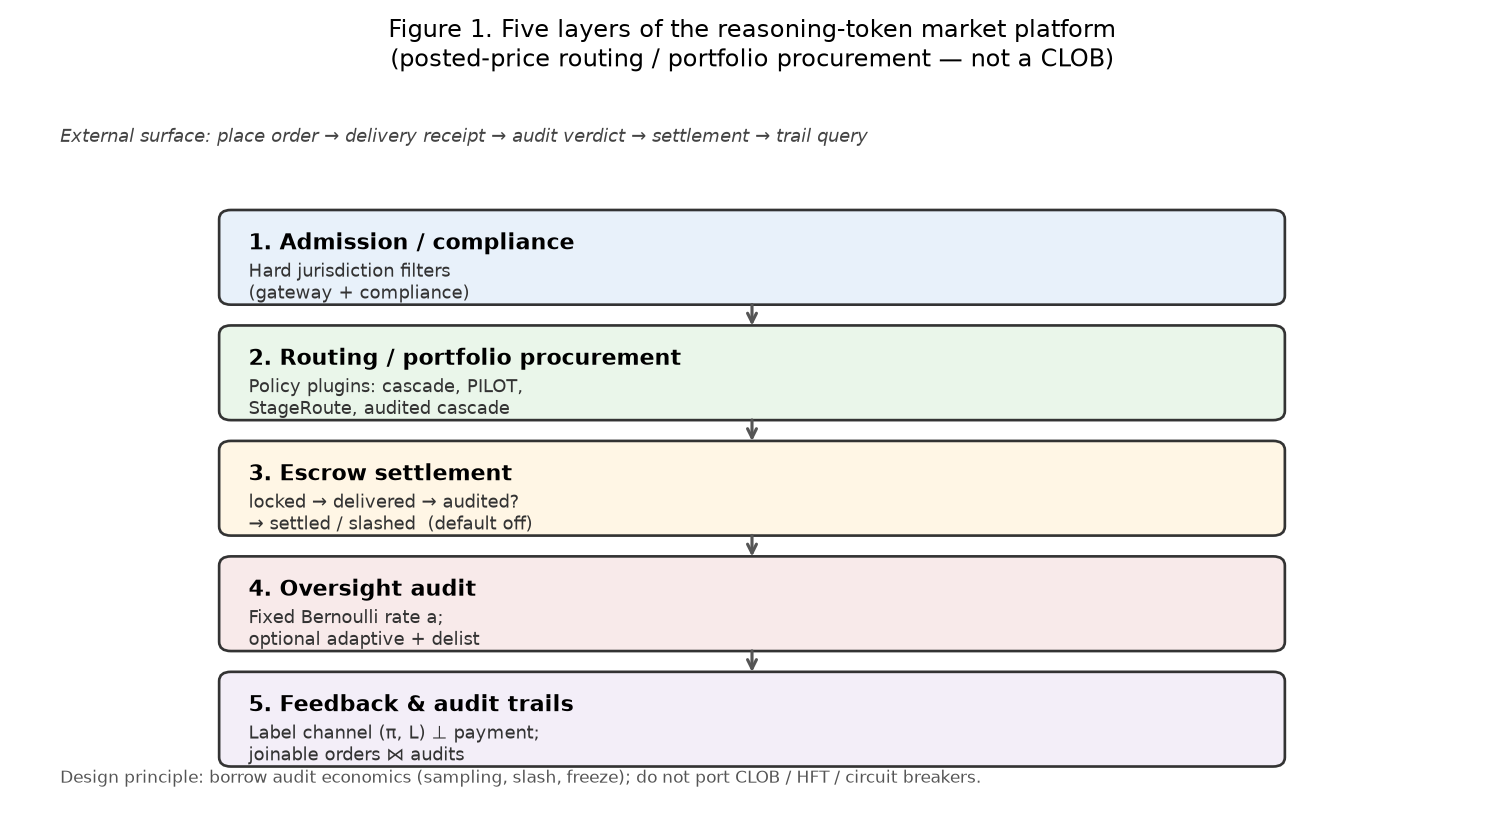
\includegraphics[width=\linewidth]{figures/fig1_five_layers.png}
  \caption{Five platform layers (admission $\rightarrow$ routing/portfolio procurement $\rightarrow$ escrow $\rightarrow$ oversight $\rightarrow$ feedback/trails). Posted-price market; not a CLOB.}
  \Description{Block diagram of the five platform layers of the reasoning-token market: admission and compliance, routing and portfolio procurement, escrow settlement, oversight, and feedback and trails.}
  \label{fig:layers}
\end{figure}

\subsection{Market primitives}
\label{sec:primitives}

\paragraph{Jurisdictions.} Synthetic CN / SG / BR corridors. Compliance profiles list allowed seller jurisdictions, sensitivity mixes, and consent rates. Rules are \emph{simplified simulations}---not legal advice (see Ethics).

\paragraph{Sellers.} Posted \code{list_price} (USD / 1k tokens), capacity per round, stake pool for slash. A strategic learning seller (\code{seller_sg} in the headline runs) chooses attack rates $q_{\mathrm{swap}}$ and $q_{\mathrm{theft}}$. Swap serves a weaker \code{actual_model} than \code{claimed_model}; theft bills more tokens than generated.

\paragraph{Buyers.} Per-buyer budgets and strategy ids. Portfolio policies may purchase from multiple sellers per task under budget.

\paragraph{Audits.} Default fixed rate $a=0.1$ with identity and length checks (detection probabilities $d_{\mathrm{identity}}=d_{\mathrm{length}}=0.9$ in headline configs) and penalty $P=0.25$. Audits update trust / slash / optional delist \textbf{immediately} and do not depend on the correctness label channel.

\paragraph{Escrow (optional).} When enabled, seller proceeds are held until the audit decision; slash is taken from the hold. Escrow is \textbf{orthogonal} to label delay $L$.

\paragraph{Delist (optional).} After a catch, \code{reputation_rounds} freezes the seller from routing until a watermark round. Default \code{reputation_rounds=0} preserves legacy F/J reproducibility.

\subsection{Design principles}
\label{sec:principles}

Borrow: sampling audits, stake slash, payment freeze, structured trails.\\
Do \textbf{not} build: CLOB, price--time priority matching, HFT makers, circuit breakers, multi-CCP. Multi-buyer congestion is deferred to Limitations.

\subsection{Joint objective (secondary)}
\label{sec:joint}

\begin{equation}
J = \mathrm{accuracy} - \lambda \cdot \mathrm{violation\_rate} - \mu \cdot \mathrm{fraud\_share},
\end{equation}
with defaults $\lambda=1.0$, $\mu=0.5$. Accuracy is task-level (portfolio answer vs gold). Violation rate is compliance breaches per task. Fraud share is attacked purchases / served purchases (\code{attack_mode} $\in$ \{\code{swap}, \code{theft}, \code{both}\}).
% TODO(pending unfreeze): primary metric redefinition
\textbf{Primary board metrics remain} \code{active_attack_rate} and \code{fraud_share}; $J$ is reported only as a scalar summary of accuracy, compliance, and fraud, and for T2's regime narrative.

%% =====================================================================
\section{Data Release}
\label{sec:data}

\subsection{Five JSONL files (v1)}
\label{sec:files}

The production boards are the reference release (schema dictionary and samples: Appendix~\ref{app:repro}). Small-scale pipeline-test exports are for pipeline testing only and are superseded by production.

\begin{table}[t]
\caption{The five JSONL files.}
\label{tab:files}
\small
\begin{tabularx}{\columnwidth}{@{}l X@{}}
\toprule
File & Role \\
\midrule
\code{sellers.jsonl} & Catalog: jurisdiction, claimed/actual model, listed quality, latent $q$, stake, ban watermark \\
\code{buyers.jsonl} & Budget, strategy\_id, compliance\_profile \\
\code{orders.jsonl} & State-machine fact table; join key \code{order_id} \\
\code{audits.jsonl} & Per served purchase: sampled checks, slash, delist, $\pi$/$L$ reveal fields \\
\code{episodes.jsonl} & \textbf{Primary board} --- one row per \code{(run_id, seed)} \\
\bottomrule
\end{tabularx}
\end{table}

\paragraph{Sample fields (production seed 0; truncated; no secrets).} Full dictionaries and three-row samples are in the schema documentation (Appendix~\ref{app:repro}).

\begin{table*}[t]
\caption{Sample fields (production seed 0; truncated; no secrets).}
\label{tab:samples}
\small
\begin{tabularx}{\textwidth}{@{}l X@{}}
\toprule
File & Compact sample keys $\rightarrow$ values \\
\midrule
\code{sellers} & \code{seller_id=seller_cn}, \code{jurisdiction=CN}, \code{claimed_model=Qwen/Qwen2.5-1.5B-Instruct}, \code{list_price=0.2}, \code{latent_q_swap=0.0} \emph{(label)}, \code{seed=0} \\
\code{buyers} & \code{buyer_id=buyer_cn_1}, \code{jurisdiction=CN}, \code{budget_total=5.0}, \code{strategy_id=audited_compliance_cascade}, \code{seed=0} \\
\code{orders} & \code{order_id=}\ldots\code{|t0000_p059|0|seller_br}, \code{state=settled}, \code{attack_mode=none} \emph{(label)}, \code{correct=false} \emph{(label)}, \code{config_hash=7b60ac28061d2907} \\
\code{audits} & \code{sampled=0}, \code{hit=0}, \code{slash_amount=0.0}, \code{reveal_pi=1.0}, \code{fraud_realized=0} \emph{(label)} \\
\code{episodes} & \code{a=0.1}, \code{pi=1.0}, \code{active_attack_rate}$\approx$0.100, \code{fraud_share}$\approx$0.100, \code{learned_q_swap}$\approx$0.042 \emph{(side)}, \code{J}$\approx$0.771 \emph{(secondary)}, \code{config_hash=7b60ac28061d2907} \\
\bottomrule
\end{tabularx}
\end{table*}

\paragraph{Join keys.} \code{run_id}, \code{seed}, \code{order_id} (= \code{purchase_id} when served), \code{config_hash} (sha256 prefix of config).

\paragraph{Derived (not shipped).} Ledger / full event timeline = \code{orders} $\bowtie$ \code{audits}. Optional \code{events} / \code{ledger} views may appear in v1.1 without changing the primary board.

\paragraph{Pipeline-test export scale.} One illustrative episode with 3 sellers, 6 buyers, 41 orders, 41 audit rows (\code{--n-tasks 48}). Full multi-seed boards used in \S\ref{sec:results} come from longer experiment configs (dense-$\pi$ sweep; delist and adaptive-audit experiments; Appendix~\ref{app:repro}).

\subsection{Feature / Label separation (application constraint)}
\label{sec:featlabel}

Several columns in the default five files are \textbf{evaluation labels}, not public training features. Using them as model inputs for fraud detection or routing ML \textbf{leaks} the supervision signal.

\begin{table}[t]
\caption{Label columns (do \textbf{not} train on).}
\label{tab:labels}
\small
\begin{tabularx}{\columnwidth}{@{}l X@{}}
\toprule
Location & Label columns (do \textbf{not} train on) \\
\midrule
\code{sellers.jsonl} & \code{actual_model}, \code{latent_q_swap}, \code{latent_q_theft} \\
\code{orders.jsonl} & \code{attack_mode}, \code{correct} \\
\code{audits.jsonl} & \code{fraud_realized}, \code{label_correct} \\
\bottomrule
\end{tabularx}
\end{table}

% TODO(pending unfreeze): §4.2 safe-feature list -- planned move of tokens_actual, audits.hit/miss/label_correct/fraud_realized, slash_amount, delist_rounds to label columns.
\paragraph{Safe public features (examples).} Jurisdictions, \code{claimed_model}, prices, capacity, stake$^{*}$, budgets$^{*}$, tokens billed/actual, amounts, \code{state}, \code{jurisdiction_path}, \code{route_policy}, audit mode/sampled/checks/hit/miss/slash/delist/auditor\_cost, reveal timing (\code{label_revealed}, \code{label_delay_L}, \code{reveal_pi}).

\paragraph{Optional held-out file.} \code{labels.jsonl} joined on \code{order_id} (\code{--with-labels}). Full public-pack stripping is deferred to \textbf{v1.1}. Until then: \textbf{do not treat the default export as a clean supervised fraud-detection training set} without dropping the label columns above.

\subsection{One-click scripts}
\label{sec:scripts}

One-click scripts export the five files and run the protocol tasks T1--T3; the exact commands are listed in Appendix~\ref{app:repro}.

Default knobs keep \code{adaptive_audit=false}, \code{reputation_rounds=0}, \code{escrow=false} so legacy F/J tables stay reproducible. Test suite: \textbf{76} tests collected and passed in-repo (\code{pytest --collect-only}; 2026-11-08 Asia/Shanghai). See Appendix~\ref{app:repro} for the reproducibility summary.

\subsection{Mechanism vs.\ model cache}
\label{sec:cache}

Correctness labels in headline ablations come from \textbf{cached real Qwen outputs} (no new generation in those runs). Feedback timing $(\pi, L)$, audits, seller learning, prices, and budgets are \textbf{simulated}. Publishable docs must keep this split explicit so downstream users do not mistake mechanism fields for organic production logs.

%% =====================================================================
\section{Benchmark Protocol}
\label{sec:protocol}

Seeds for headline tables: $\{0,1,2\}$. Budget multiplier $2.0$. Strategic seller attack modes \{\code{swap}, \code{theft}\}. Audit rate $a=0.1$ on audited arms.

\subsection*{T1 --- Fixed-$a$ deterrence (primary)}

\paragraph{Goal.} Measure whether fixed-rate oversight compresses seller attack intensity and realized fraud relative to non-auditing routers.

% TODO(pending unfreeze): primary metric redefinition
\paragraph{Primary metrics.} Split attack-rate definitions so they stay consistent with \S\ref{sec:delist} and production \code{episodes.jsonl}: (i) \textbf{\code{active_attack_rate}} = active trade attack rate = attacked / served purchases (\code{status=allowed}); (ii) \textbf{\code{learned_q_swap} / \code{learned_q_theft}} = epoch-mean learned $q$ on the strategic seller (separate columns). Without delist the two are close (production T1 means $\approx$0.101 vs $\approx$0.083/0.081); with delist they can diverge (learned $q$ may rise from missing observations while active-trade attack rate falls). 
% TODO(pending unfreeze): primary metric redefinition
Board also reports \code{fraud_share} (same formula as active\_attack\_rate in v1 production). Always list both attack columns when \code{reputation_rounds>0}.

% TODO(pending unfreeze): D3 presented as the paper's method (listed among T1 arms) -- planned relabel 'fixed-audit-rate baseline'.
\paragraph{Baselines.} StageRoute+compliance, PILOT+compliance (audit rate 0); fixed-$a$ D3 (\code{audited_compliance_cascade}); random audit on a simple compliant selector.

% TODO(pending unfreeze): primary metric redefinition
\paragraph{Reading rule.} Rank primarily by attack/fraud, not by immediate-feedback $J$.

\subsection*{T2 --- Sparse-label regime (primary protocol result)}

% TODO(pending unfreeze): 'D3 insensitive to pi' sentence ("deterrence (q*) stays audit-driven and pi-invariant") -- planned deletion.
\paragraph{Goal.} Sweep reveal probability $\pi$ at delay $L=0$ and locate where sparse labels flip the \emph{secondary} $J$ ordering between D3 and the best compliant bandit---interpreted as \textbf{bandit collapse under missing labels}, while deterrence ($\qstar$) stays audit-driven and $\pi$-invariant.

\paragraph{Grid (dense).} $\pi \in \{1.0,\allowbreak 0.2,\allowbreak 0.18,\allowbreak 0.15,\allowbreak 0.12,\allowbreak 0.10,\allowbreak 0.08,\allowbreak 0.06,\allowbreak 0.05,\allowbreak 0.0\}$ (configuration and results: Appendix~\ref{app:repro}).

% TODO(pending unfreeze): pi* (0.10,0.12) statement -- planned rewrite to a conditional interval with per-seed spread.
\paragraph{Summary of findings.} The crossover lies at $\pistar \in (0.10, 0.12)$; this does \textbf{not} mean that D3 wins under full feedback.

\subsection*{T3 --- Audit-cost efficiency (appendix only)}

\paragraph{Goal.} Same expected audit budget: fixed Bernoulli vs risk-targeted adaptive allocation; report fraud / $J$ / \code{n_audits}. \textbf{Not} primary novelty; \textbf{not} a full comparison against instantaneous bandits.

\paragraph{Delist ablation (appendix).} Sweep \code{reputation_rounds} $\in \{0,5,20\}$; always report \textbf{both} realized fraud share and learned $q$ (delist can cut fraud while raising epoch-mean learned $q$ via missing observations).

%% =====================================================================
\section{Platform Capability Results}
\label{sec:results}

Numbers below are taken from the released experiment artifacts and the production one-click boards (seeds $\{0,1,2\}$, \code{n_tasks=480}; paths in Appendix~\ref{app:repro}). Small-scale pipeline-test runs use short task counts and \textbf{do not} replace these tables.

\subsection{T1 --- Fixed-$a$ deterrence (from joint / feedback tables)}
\label{sec:t1}

Under immediate full feedback ($\pi=1$, $L=0$), seeds $\{0,1,2\}$, budget $\times 2$, swap+theft learning seller (dense-feedback ablation, consistent with the immediate-feedback $J$ ranking; Appendix~\ref{app:repro}):

%% Column order (team decision): primary board first, side columns, J last.
%% active_attack_rate values: release/v0.1/results/benchmark/production/T2_episodes.jsonl
%%   (pi=1.0, L=0, seeds {0,1,2}, mean +- sample sd); D3 row also matches T1_episodes.jsonl.
%%   In v1 production active_attack_rate == fraud_share (same formula; see Sec. 5).
% TODO(pending unfreeze): D3 row is bold-highlighted (presented like the paper's method) -- planned relabel 'fixed-audit-rate baseline'.
% TODO(pending unfreeze): primary metric redefinition
\begin{table*}[t]
\caption{T1 under immediate full feedback ($\pi=1$, $L=0$), seeds $\{0,1,2\}$. Primary-board columns first; learned $q$ side columns; $J$ (secondary) last.}
\label{tab:t1}
\small
\begin{tabular}{@{}lcccc@{}}
\toprule
Policy & \code{active_attack_rate} & \code{fraud_share} & Learned $q_{\mathrm{swap}}/q_{\mathrm{theft}}$ (side) & $J$ (secondary) \\
\midrule
StageRoute+compliance & $0.023 \pm 0.022$ & $0.023 \pm 0.022$ & $0.80 / 0.77$ & $0.811 \pm 0.026$ \\
PILOT+compliance & $0.045 \pm 0.011$ & $0.045 \pm 0.011$ & $0.95 / 0.93$ & $0.789 \pm 0.010$ \\
\textbf{D3 fixed $a=0.1$} & $0.101 \pm 0.023$ & $0.101 \pm 0.023$ & $\mathbf{0.08 / 0.08}$ & $0.766 \pm 0.037$ \\
\bottomrule
\end{tabular}
\end{table*}

% TODO(pending unfreeze): primary metric redefinition
% TODO(pending unfreeze): D3 presented as the paper's method ("Primary board therefore favors D3") -- planned relabel 'fixed-audit-rate baseline'.
\paragraph{Reading.} At $\pi=1$, on the primary column \texttt{fraud\_share} the bandits are lower (StageRoute 0.023, PILOT 0.045, D3 0.101) because they avoid attackers; D3 leads only on the side column learned $q$ (about 0.08 vs.\ 0.77--0.95 for the bandits).

% TODO(pending unfreeze): primary metric redefinition
\paragraph{Production export.} The one-click production board (\code{episodes.jsonl}; paths in Appendix~\ref{app:repro}) uses seeds $\{0,1,2\}$, \code{n_tasks=480}, \code{n_rounds=48}, learning swap+theft, adaptive audit, delist, and escrow disabled (defaults), cache-backed sellers. Mean over seeds: \code{active_attack_rate=fraud_share}$\approx$0.101, \code{learned_q_swap}$\approx$0.083, \code{learned_q_theft}$\approx$0.081, \code{J}$\approx$0.766, \code{n_audits}$\approx$60.3---aligned with the dense-$\pi$ sweep and the delist/adaptive-audit experiments. The 48-task pipeline-test export is for pipeline testing only and is not used as the board. Terminology: \code{active_attack_rate} is attacked/served purchases; \code{learned_q_*} are separate columns.

\subsection{T2 --- Sparse $\pi$ regime and $\pistar$}
\label{sec:t2}

Dense $L=0$ sweep:

%% Layout differs from Table T1 (a per-pi J sweep that defines the crossover);
%% column order kept exactly as in the draft.
\begin{table*}[t]
\caption{T2 dense $L=0$ sweep over reveal probability $\pi$.}
\label{tab:t2}
\small
\begin{tabular}{@{}rccccccc@{}}
\toprule
$\pi$ & PILOT $J$ & StageRoute $J$ & D3 $J$ & $\Delta J=$ D3 $-$ best bandit & D3 $q_{\mathrm{swap}}/q_{\mathrm{theft}}$ & Best-bandit $q_{\mathrm{swap}}/q_{\mathrm{theft}}$ \\
\midrule
1.0 & 0.789 & 0.811 & 0.766 & $-0.045$ & 0.08 / 0.08 & 0.80 / 0.77 \\
0.20 & 0.780 & 0.803 & 0.766 & $-0.037$ & 0.08 / 0.08 & 0.64 / 0.61 \\
0.18 & 0.763 & 0.799 & 0.766 & $-0.033$ & 0.08 / 0.08 & 0.64 / 0.61 \\
0.15 & 0.772 & 0.798 & 0.766 & $-0.031$ & 0.08 / 0.08 & 0.64 / 0.61 \\
0.12 & 0.729 & 0.789 & 0.766 & $-0.023$ & 0.08 / 0.08 & 0.80 / 0.77 \\
\textbf{0.10} & 0.726 & 0.747 & 0.766 & $\mathbf{+0.019}$ & 0.08 / 0.08 & 0.95 / 0.94 \\
0.08 & 0.699 & 0.737 & 0.766 & $+0.029$ & 0.08 / 0.08 & 0.95 / 0.94 \\
0.06 & 0.652 & 0.714 & 0.766 & $+0.052$ & 0.08 / 0.08 & 0.95 / 0.94 \\
0.05 & 0.673 & 0.681 & 0.766 & $+0.085$ & 0.08 / 0.08 & 0.95 / 0.94 \\
0.0 & $-0.030$ & 0.585 & 0.766 & $+0.181$ & 0.08 / 0.08 & 0.95 / 0.94 \\
\bottomrule
\end{tabular}
\end{table*}

% TODO(pending unfreeze): pi* (0.10,0.12) statement -- planned rewrite to a conditional interval with per-seed spread.
% TODO(pending unfreeze): 'D3 insensitive to pi' sentence ("D3's q* is constant across pi") -- planned deletion.
\paragraph{Crossover.} On this grid, $\Delta J < 0$ at $\pi=0.12$ and $\Delta J > 0$ at $\pi=0.10$, hence $\boldsymbol{\pistar \in (0.10, 0.12)}$. D3's $\qstar$ is \textbf{constant across $\pi$} (audits independent of outcome feedback). Compliant bandits never compress $q$; under $\pi \le 0.10$ their learned attack rates rise to $\approx 0.95$, i.e., avoidance fails when labels vanish.

% TODO(pending unfreeze): pi* (0.10,0.12) statement (production T2) -- planned rewrite to a conditional interval with per-seed spread.
\paragraph{Production T2.} The production T2 run (dense grid identical to the sweep above) reports $\pistar_J \in (0.10, 0.12)$ with $\Delta J(0.12)\approx -0.023$ and $\Delta J(0.10)\approx +0.019$, matching the dense sweep. A coarse pipeline-test T2 run is for pipeline testing only and is not reported.

% TODO(pending unfreeze): pi* (0.10,0.12) statement in Fig. 2 caption -- planned rewrite to a conditional interval with per-seed spread.
% TODO(pending unfreeze): primary metric redefinition (Fig. 2 caption)
% TODO(pending unfreeze): 'D3 insensitive to pi' sentence in Fig. 2 caption ("fixed-a D3 stays near 0.08 across pi") -- planned deletion.
\begin{figure*}[t]
  \centering
  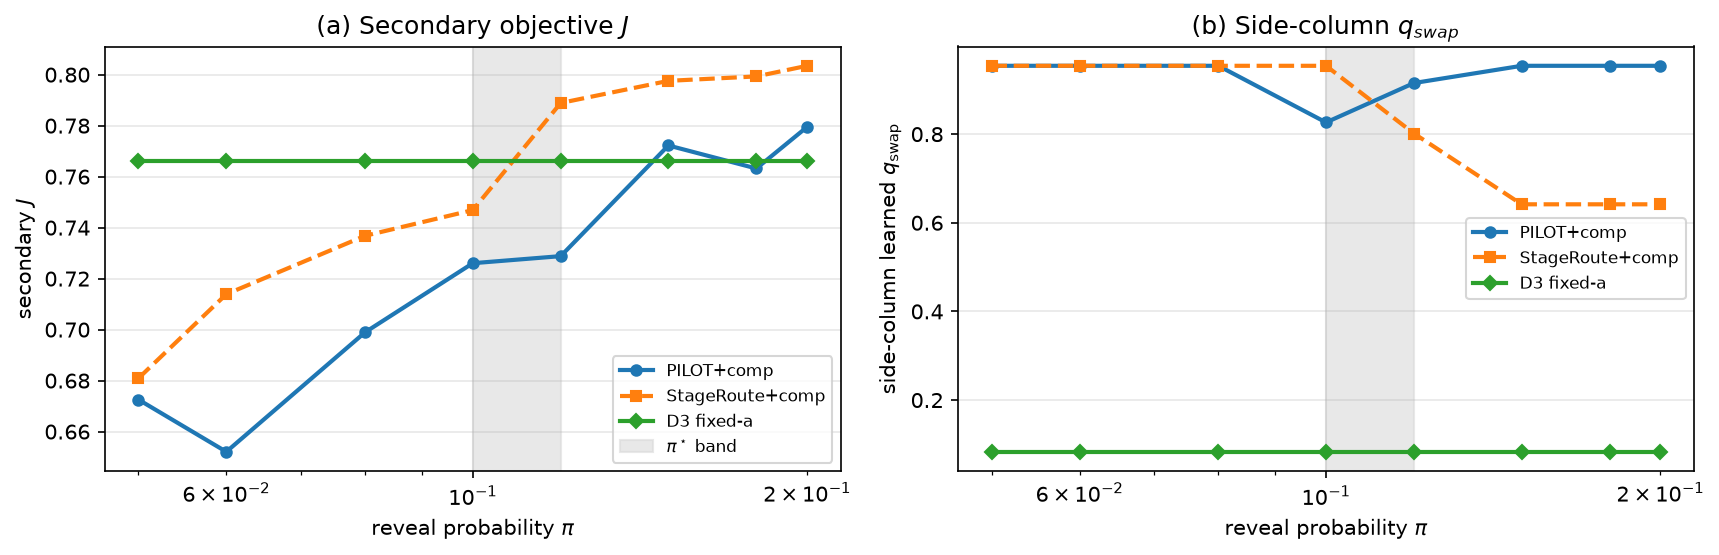
\includegraphics[width=\textwidth]{figures/fig2_pi_star_crossover.png}
  \caption[T2 $\pi$ sweep at $L=0$ and the $\pistar$ crossover.]{T2 $\pi$ sweep at $L=0$. \textbf{(a)} Secondary $J$: bandits dominate under dense labels; D3 overtakes between $\pi=0.12$ and $\pi=0.10$ ($\pistar \in (0.10,0.12)$). \textbf{(b)} Side-column learned $q_{\mathrm{swap}}$: fixed-$a$ D3 stays near $0.08$ across $\pi$; compliant bandits never compress $\qstar$ (avoidance collapses as labels vanish). \textbf{Not} a claim that D3 beats PILOT/StageRoute on $J$ under full feedback; primary board remains \code{active_attack_rate} + \code{fraud_share}. Seeds $\{0,1,2\}$; the crossover is confirmed by the production T2 run. The production episodes export holds the fixed-$\pi{=}1$ board rows (\code{config_hash=7b60ac28061d2907}); the full $\pi$ grid lives in the dense-sweep and production T2 artifacts, not in a single episodes export (Appendix~\ref{app:repro}).}
  \Description{Two-panel line chart over reveal probability pi. Panel (a) shows the secondary joint objective J for PILOT, StageRoute, and D3, with D3 overtaking the bandits between pi = 0.12 and pi = 0.10. Panel (b) shows learned q_swap, with D3 near 0.08 and the bandits high.}
  \label{fig:pistar}
\end{figure*}

\subsection{Appendix --- Delist trade-off}
\label{sec:delist}

Policy D3, $a=0.1$, seeds $\{0,1,2\}$:

\begin{table}[t]
\caption{Delist trade-off, policy D3, $a=0.1$.}
\label{tab:delist}
\small
\setlength{\tabcolsep}{2.5pt}
\begin{tabular}{@{}ccccc@{}}
\toprule
\makecell{\code{reputation_}\\\code{rounds}} & Learned $q_{\mathrm{swap}}$ & $J$ & Fraud share & $n_{\mathrm{audits}}$ \\
\midrule
0 & $0.083 \pm 0.049$ & $0.766 \pm 0.037$ & $0.101 \pm 0.023$ & 60.3 \\
5 & $0.181 \pm 0.136$ & $0.787 \pm 0.010$ & $0.063 \pm 0.006$ & 57.7 \\
20 & $0.439 \pm 0.427$ & $0.807 \pm 0.019$ & $0.041 \pm 0.022$ & 55.0 \\
\bottomrule
\end{tabular}
\end{table}

\paragraph{Reading.} Longer delist \textbf{cuts realized fraud} and lifts $J$, but epoch-mean learned $q$ can \textbf{rise} because banned sellers contribute fewer post-slash observations. Report both metrics; do not claim delist alone drives $\qstar \to 0$. Default remains \code{reputation_rounds=0}.

\subsection{Appendix --- Adaptive audit under equal expected budget}
\label{sec:adaptive}

Same target $a=0.1$, escrow on:

\begin{table}[t]
\caption{Adaptive audit under equal expected budget.}
\label{tab:adaptive}
\small
\setlength{\tabcolsep}{2.5pt}
\begin{tabular}{@{}lccccc@{}}
\toprule
Arm & $q_{\mathrm{swap}}$ & $J$ & \makecell{Fraud\\share} & $n_{\mathrm{audits}}$ & \makecell{Realized\\$a$} \\
\midrule
Fixed & $0.083 \pm 0.049$ & $0.766 \pm 0.037$ & $0.101 \pm 0.023$ & 60.3 & 0.087 \\
Adaptive & $0.056 \pm 0.035$ & $0.803 \pm 0.019$ & $0.044 \pm 0.009$ & 66.0 & 0.099 \\
\bottomrule
\end{tabular}
\end{table}

Escrow flows (fixed / adaptive): held $12.26 / 11.47$, slashed $0.15 / 0.23$, released $12.11 / 11.24$. \textbf{Reading.} Adaptive targeting is a cost/aiming improvement under a comparable audit count---not a claim of dominance over instantaneous bandits, and not primary novelty.

%% =====================================================================
\section{Limitations}
\label{sec:limitations}

\begin{enumerate}
\item \textbf{Single-platform auditor; no multi-buyer congestion.} Multi-buyer competition for capacity and multi-auditor games are deferred (explicit limitation, not a silent omission). Congestion externalities are therefore out of the v1 leaderboard contract.
\item \textbf{Not a CLOB.} Posted prices + routing/portfolio procurement only; no price--time priority book, maker--taker fees, HFT makers, or circuit breakers. Exchange-microstructure claims are out of scope.
\item \textbf{Synthetic jurisdictions and mechanism + cached model answers.} Corridor tags (CN/SG/BR) and compliance profiles are simplified simulation devices---not legal advice and not real KYC/data-transfer regimes. Correctness may come from cached Qwen generations; prices, budgets, audits, and learning rules are simulated. Fields should not be treated as organic production telemetry.
\item \textbf{Feature/Label hygiene for fraud detectors.} \code{attack_mode} / \code{correct} / \code{actual_model} / \code{latent_q_*} ship in the default five files for leaderboard joins; they are \textbf{evaluation labels}, not public training features. Supervised fraud-detection or routing ML that trains on them silently leaks supervision. Prefer dropping those columns or joining the optional held-out \code{labels.jsonl} (full public-pack strip deferred to v1.1).
\item \textbf{Adaptive audit \& long delist are optional knobs}, not claimed SOTA over instantaneous bandits on secondary $J$, and not primary novelty of this Datasets \& Benchmarks paper.
\item \textbf{Pipeline-test vs.\ full boards.} Small-scale pipeline-test exports are for pipeline testing only. The released v0.1 downloadable board (paths in Appendix~\ref{app:repro}) matches the seed-mean tables of the dense-$\pi$ sweep and the delist/adaptive-audit experiments.
\item \textbf{No resale / rewrite / distill event graph.} v0.1 has no \code{event_type}$\in$\{\code{resale},\code{rewrite},\code{distill}\} layer, no \code{parent_order_id} / \code{source_order_id} / \code{downstream_model_id}, and no content/output hashes. Strong provenance and cross-border reuse RQs are deferred to a v1.1 event layer---not claimed here.
% TODO(pending unfreeze): primary metric redefinition
\item \textbf{Primary metrics.} Leaderboard ranking uses \code{active_attack_rate} + \code{fraud_share} only. \code{learned_q_*} are side columns; immediate-feedback $J$ (incl.\ vs PILOT/StageRoute) is secondary and is not the primary ranking. No deterrence-method novelty is claimed.
\end{enumerate}

%% =====================================================================
\section{Conclusion}
\label{sec:conclusion}

% TODO(pending unfreeze): pi* (0.10,0.12) statement -- planned rewrite to a conditional interval with per-seed spread.
% TODO(pending unfreeze): primary metric redefinition
We release a \textbf{compliance-constrained reasoning-token market simulator}---a \textbf{generator + protocol + downloadable board}, not a new routing method---for procurement under strategic fraud and sparse audit feedback. The platform is deliberately \emph{not} a CLOB: it exposes admission, routing, escrow, oversight, and feedback trails as a joinable five-file export. Primary leaderboard metrics are \textbf{\code{active_attack_rate} + \code{fraud_share}} only; \code{learned_q_*} remain side columns; immediate-feedback $J$ (including comparisons to PILOT / StageRoute) is secondary and is \textbf{not} the primary ranking. Sparse-label regime structure ($\pistar \in (0.10, 0.12)$) is a protocol result about bandit collapse under missing labels, not a claim of beating PILOT on $J$. Designing deterrence or audit methods that improve on this board is left to future methods work. We invite Datasets \& Benchmarks submissions and leaderboard entries on T1--T2, with T3 and delist kept as cost/ops appendices, and with Feature/Label hygiene enforced for downstream application analysis.

%% =====================================================================
\section*{Ethics and Synthetic-Data Statement}
\label{sec:ethics}

All market prices, budgets, stakes, corridor fees, and compliance rule identifiers are \textbf{synthetic}. Jurisdiction labels (CN/SG/BR) and rule tags are simplified simulation devices and \textbf{do not constitute legal advice}. Default runs do not call external commercial APIs or require API keys; optional local small-model backends and cached Qwen outputs are research fixtures. The benchmark is intended for studying procurement, audit, and feedback protocols---not for training systems to evade real-world marketplace detection. Users building fraud classifiers must respect the Feature/Label separation in \S\ref{sec:featlabel} to avoid leakage and overstated detection performance.

%% =====================================================================
%% References. The draft's human-readable key map lists two entries that
%% are not cited in the text (bester2001strategic, cumming2019capital);
%% they are \nocite'd so the rendered list matches that map.
%% Remove the \nocite line if only in-text citations should be listed.
\nocite{bester2001strategic,cumming2019capital}
\bibliographystyle{ACM-Reference-Format}
\bibliography{refs}

%% =====================================================================
\appendix

\section{Schema field cheat-sheet}
\label{app:schema}

See \code{docs/DATA_SCHEMA.md} for full dictionaries and three-row samples. Minimal primary-board row (\code{episodes.jsonl}):
% TODO(pending unfreeze): primary metric redefinition

\code{run_id, seed, a, pi, L, reputation_rounds, active_attack_rate, learned_q_swap, learned_q_theft, fraud_share, J, n_audits, config_hash}.

\section{Reproducibility and Artifact Paths}
\label{app:repro}

All repository and file paths referenced by the main text are collected here. The release pack \code{release/v0.1/} mirrors \code{exports/production/} and \code{results/benchmark/production/}; small-scale pipeline-test outputs (\code{exports/latest/}, top-level \code{results/benchmark/}) are for pipeline testing only.

\paragraph{One-click scripts.}
\begin{lstlisting}
# Pipeline test (-> exports/latest/)
python scripts/export_benchmark_layers.py --out exports/latest --seed 0 --n-tasks 48 --learning

# Production board (-> exports/production/)
python scripts/export_benchmark_layers.py --full --use-cache --out exports/production

# Protocol tasks T1-T3 (production scale)
python scripts/run_benchmark_tasks.py --full --use-cache
python scripts/run_leaderboard.py --smoke   # optional pipeline-test board
\end{lstlisting}

\begin{table*}[h]
\caption{Reproducibility summary.}
\label{tab:repro}
\small
\begin{tabularx}{\textwidth}{@{}l X@{}}
\toprule
Item & Value / path \\
\midrule
Downloadable data pack & \code{release/v0.1/} (\code{SHA256SUMS}, \code{MANIFEST.json}, \code{REPRODUCE.md}) \\
One-click pipeline-test export & \code{python scripts/export_benchmark_layers.py --out exports/latest --seed 0 --n-tasks 48 --learning} \\
One-click production export & \code{python scripts/export_benchmark_layers.py --full --use-cache --with-labels} \\
Protocol tasks & \code{python scripts/run_benchmark_tasks.py --full --use-cache} \\
Production board path & \code{release/v0.1/exports/production/}\{\code{sellers},\code{buyers},\code{orders},\code{audits},\code{episodes},\code{labels}\}\code{.jsonl} (mirrors \code{exports/production/}) \\
Production T1--T3 & \code{release/v0.1/results/benchmark/production/} \\
Pipeline-test output & \code{exports/latest/} (not used for reported tables) \\
Headline seeds & $\{0,1,2\}$; production episodes use these three \\
Production \code{config_hash} & \code{7b60ac28061d2907} (on every \code{orders} / \code{episodes} row) \\
Dense $\pi$ grid config & \code{configs/pi_dense.yaml} $\rightarrow$ \code{results/pi_dense/} (also under \code{release/v0.1/}) \\
Feature/Label rules & \code{docs/DATA_SCHEMA.md} \S Feature/Label (+ \S\ref{sec:featlabel}); copy in \code{release/v0.1/docs/} \\
Default knobs & \code{adaptive_audit=false}, \code{reputation_rounds=0}, \code{escrow=false} \\
Test suite & \textbf{76} collected / \textbf{76 passed} (\code{results/benchmark/pytest_after_draft.txt}, 2026-11-08 Asia/Shanghai) \\
\bottomrule
\end{tabularx}
\end{table*}

\begin{table}[h]
\caption{Platform layer code map.}
\label{tab:codemap}
\small
\begin{tabularx}{\columnwidth}{@{}l X@{}}
\toprule
Layer & Code map \\
\midrule
1. Admission / compliance & \code{gateway.py}, \code{compliance.py} \\
2. Routing / portfolio & \code{matching.py}, \code{portfolio.py}, \code{buyers.py}, \code{baselines.py} \\
3. Escrow settlement & \code{sim.py}, \code{audit_v6.py} \\
4. Oversight & \code{strategic.py}, \code{audit_v6.py} \\
5. Feedback \& trails & \code{feedback.py}, \code{logging_schema.py} \\
\bottomrule
\end{tabularx}
\end{table}

\begin{table*}[h]
\caption{Source artifact paths.}
\label{tab:paths}
\small
\begin{tabularx}{\textwidth}{@{}l X@{}}
\toprule
Item & Path \\
\midrule
Dense $\pi$ grid config & \code{configs/pi_dense.yaml} $\rightarrow$ \code{results/pi_dense/} \\
Fig.~\ref{fig:pistar} data & \code{results/pi_dense/feedback_ablation.json}; production crossover \code{results/benchmark/production/T2_crossover.json} \\
T1 production episodes & \code{exports/production/episodes.jsonl}, \code{results/benchmark/production/T1_episodes.jsonl} \\
Figure art & \code{docs/figures/fig1_five_layers.}\{\code{png},\code{svg}\}, \code{docs/figures/fig2_pi_star_crossover.}\{\code{png},\code{svg}\} \\
Paper outline & \code{docs/BENCHMARK_PAPER_OUTLINE.md} \\
Schema + Feature/Label & \code{docs/DATA_SCHEMA.md} \\
Dense $\pistar$ tables & \code{results/pi_dense/feedback_ablation.md}, \code{SUMMARY_zh.txt} \\
Immediate-feedback $J$ ranking & \code{results/joint_objective.md} \\
Delist appendix & \code{results/v6_delist.md}, \code{v6_delist.json} \\
Adaptive appendix & \code{results/v6_adaptive_audit.md}, \code{v6_adaptive_audit.json} \\
Delist/adaptive-audit summary & \code{results/v6_SUMMARY_zh.txt} \\
Release pack (download) & \code{release/v0.1/} (+ \code{SHA256SUMS}, \code{MANIFEST.json}, \code{REPRODUCE.md}) \\
Production export & \code{release/v0.1/exports/production/*.jsonl} (mirrors \code{exports/production/}) \\
Production T1--T3 & \code{release/v0.1/results/benchmark/production/} \\
Production summary & \code{release/v0.1/results/benchmark/PRODUCTION_EXPORT_zh.txt} \\
Test log & \code{results/benchmark/pytest_after_draft.txt} (76 passed) \\
Pipeline-test export & \code{exports/latest/*.jsonl} \\
Pipeline-test T1--T3 & \code{results/benchmark/} (top-level) \\
\bottomrule
\end{tabularx}
\end{table*}

Clone $\rightarrow$ open \code{release/v0.1/} (or re-run the two one-click commands) $\rightarrow$ read \code{episodes.jsonl} should recover Table~\ref{tab:t1} means and the $\pistar$ narrative without re-tuning.

\section{RQ coverage (v0.1 vs v1.1)}
\label{app:rq}

This appendix maps nearby research questions onto the released v0.1 pack. It \textbf{does not} expand the paper's primary claims: the contribution remains the generator + T1--T3 protocol; primary board metrics remain \code{active_attack_rate} + \code{fraud_share}.
% TODO(pending unfreeze): primary metric redefinition

% TODO(pending unfreeze): primary metric redefinition
\begin{table*}[h]
\caption{RQ coverage (v0.1 vs v1.1).}
\label{tab:rq}
\footnotesize
\setlength{\tabcolsep}{3pt}
\begin{tabularx}{\textwidth}{@{}>{\raggedright\arraybackslash}p{2.3cm} >{\raggedright\arraybackslash}X >{\raggedright\arraybackslash}p{2.4cm} >{\raggedright\arraybackslash}p{2.5cm} >{\raggedright\arraybackslash}p{2.9cm} >{\raggedright\arraybackslash}p{3.2cm}@{}}
\toprule
RQ & Example task & Inputs & Labels / supervision & Metrics & Coverage \\
\midrule
\textbf{T1--T3 (protocol)} & Fixed-$a$ deterrence; $\pistar$ regime; equal-budget adaptive (appendix) & \code{episodes} (+\code{orders}/\code{audits}) & episode eval only & \code{active_attack_rate}, \code{fraud_share} (primary); \code{n_audits} for T3 & \textbf{v0.1} \\
\textbf{A2 multi-jurisdiction compliance} & Hard-filter violation / route reachability & \code{buyers}+\code{orders}(+\code{sellers}) & path $\times$ \code{compliance_profile} (derived) & violation rate, fill rate & \textbf{v0.1 enough (basic)} --- not a full regulatory rule library \\
\textbf{A1 provenance (weak)} & Order $\rightarrow$ claimed/actual model $\rightarrow$ audit trail & \code{orders}$\bowtie$\code{audits}$\bowtie$\code{sellers} & \code{labels.actual_model} (held-out) & trail completeness; weak ID accuracy & \textbf{v0.1 weak} --- trade/audit trail only \\
\textbf{A1 provenance (strong)} & Content-level provenance chain & needs hashes + parent links & content/output match & provenance-chain accuracy & \textbf{v1.1} \\
\textbf{C1 market mechanism} & Posted-price + audit-rate protocols & \code{orders}+\code{episodes}+\code{audits} & episode eval & attack/fraud, volume, \code{n_audits} & \textbf{v0.1 partial} (posted-price only; \textbf{no auction}) \\
\textbf{C1 auctions} & Bid / clear / allocate & needs mechanism fields & allocation labels & efficiency, revenue & \textbf{v1.1} \\
\textbf{Resale / rewrite / distill} & Downstream reuse of upstream inference & needs event layer & \code{source_order_id}, \code{downstream_model_id} & provenance-chain match & \textbf{v1.1 gap} \\
\bottomrule
\end{tabularx}
\end{table*}

\paragraph{v0.1 already has:} \code{jurisdiction_path}, \code{claimed_model}/\code{actual_model}, \code{attack_mode}, \code{tokens_billed}/\code{tokens_actual}, audit trail, \code{compliance_profile}, \code{config_hash}.

\paragraph{Deferred to v1.1 event layer (do not silently claim in v0.1):} \code{content_hash}/\code{prompt_hash}/\code{output_hash}, \code{parent_order_id}, \code{provenance_depth}, \code{event_type}$\in$\{\code{resale},\code{rewrite},\code{distill}\}, \code{source_order_id}, \code{downstream_model_id}, \code{mechanism}$\in$\{\code{posted},\code{auction}\}, \code{bid}/\code{clearing_price}/\code{allocation}, explicit \code{rule_id}/\code{violation_code}.

%% =====================================================================
%% Draft "References" key->title map (human-readable; refs.bib is authoritative):
%%   becker1968crime            Becker (1968), Crime and Punishment
%%   avenhaus2002inspection     Avenhaus, von Stengel & Zamir (2002), Inspection Games
%%   daughety2008communicating  Daughety & Reinganum (2008), Communicating Quality
%%   bester2001strategic        Bester & Ritzberger (2001), Strategic Pricing... (lineage)
%%   bester2021signaling        Bester, Lang & Li (2021), Signaling versus Auditing
%%   hanson2003combinatorial    Hanson (2003), Combinatorial Information Market Design
%%   wolfers2004prediction      Wolfers & Zitzewitz (2004), Prediction Markets
%%   uma2024optimistic          UMA docs - How Does UMA Resolve Prediction Markets?
%%   polymarket2024resolution   Polymarket docs - Resolution
%%   panda2025pilot             Panda et al. (2025), Adaptive LLM Routing... (PILOT; EMNLP Findings)
%%   li2026stageroute           Li & Li (2026), Near-Optimal... Streaming LLMs (StageRoute; ICLR)
%%   iosco2009surveillance      IOSCO (2009), Approaches to Market Surveillance...
%%   cumming2008surveillance    Cumming & Johan (2008), Global Market Surveillance
%%   cumming2019capital         Cumming & Johan (2019), Capital-Market Effects... (related)
%%   aws2024compute_sla         AWS Compute SLA (industry-practice placeholder)
%%
%% Draft camera-ready checklist (kept as comments; not part of the paper body):
%%   [x] BibTeX in docs/refs.bib; Related Work uses pandoc [@key] (now \cite)
%%   [x] Abstract primary metrics = active_attack_rate + fraud_share; learned_q_* side columns; no "beat PILOT on J" ranking
%%   [x] Production boards cited via release/v0.1/ (mirrors exports/production/, results/benchmark/production/); exports/latest/ illustrative only
%%   [x] Self-contained: no companion-paper dependency; no deterrence-method novelty claimed (2026-11-10)
%%   [x] Figure 1 (five layers) + Figure 2 (pi* crossover from pi_dense / production T2)
%%   [x] Schema sample table + Feature/Label pointer (DATA_SCHEMA.md)
%%   [x] Reproducibility one-pager (Sec. 6.5): export commands, seed, config_hash, test count (76)
%%   [x] Limitations expanded (multi-buyer, non-CLOB, single auditor, Feature/Label hygiene, synthetic jurisdictions, no resale/rewrite/distill graph)
%%   [x] Appendix C RQ coverage (v0.1 vs v1.1); claims not expanded
%%   [ ] Final venue formatting / camera-ready PDF styling; confirm StageRoute ICLR 2026 pagination when proceedings land
%% Draft v0.1 camera-ready polish 2026-11-08 (Asia/Shanghai): Fig.1/Fig.2; claim sweep; repro one-pager; schema samples; production paths authoritative.
\end{document}
